\section{From Typed to Untyped Universes}

\subsection{Organizing Untyped Universes}
"Por que os tipos são necessários para  as LPs", para responder a essa pergunta, examinamos como os tipos surgem em vários domínios da ciência da computação e da matemática.
Para isso, vamos repartir esse universo em 4 partes.
\begin{itemize}
    \item Strings de bits na memória do computador:
    \item Expressões-S em LISP puro:
    \item Expressões $\lambda$ em calculo $\lambda$:
    \item Conjunto da teoria de conjuntos:
\end{itemize}
\subsubsection{\textit{Bit strings}}
O mais concreto dos tipos. Considerado “não tipado”, porém representado como cadeias de bits: caracteres, números, ponteiros, dados estruturados, programas.
O pedaço de memória bruta, geralmente não temos como dizer o que está sendo representado este significado é dado por um interpretador externo.

\subsubsection{Puro LISP}
As expressões S de LISP formam outro universo não tipado, que geralmente é construído em cima do universo de \textit{string} de bits anterior. Programas e dados não são distinguidos e, por fim, tudo é uma expressão S de algum tipo.
Novamente, temos apenas um tipo, embora seja um pouco mais estruturado e tenha melhores propriedades do que cadeias de bits.

\subsubsection{Calculo $\lambda$}
No cálculo $\lambda$, tudo é uma função. Números, estruturas de dados e até cadeias de bits podem ser representados por funções apropriadas.

\subsubsection{Teoria de conjuntos}
Na teoria dos conjuntos, tudo é um elemento ou um conjunto de elementos e/ou outros conjuntos.
Por exemplo, os inteiros são geralmente representados por conjuntos de conjuntos cujo nível de aninhamento representa a cardinalidade do inteiro, enquanto as funções são representadas por conjuntos possivelmente infinitos de pares ordenados com primeiros componentes únicos.

\subsection{Static and Strong Typing}

Um tipo é um conjunto de regras que restringem a maneira como os objetos podem interagir com outros objetos, por exemplo, objetos de tipos diferentes não podem interagir entre sí.
Para evitar violações de tipo, geralmente impomos uma estrutura de tipos estática aos programas. 
Linguagens de programação nas quais o tipo de cada expressão pode ser determinado por análise estática de programa são ditas estaticamente tipadas.
A tipagem estática é uma propriedade útil, mas, ha o requisito de que todas as variáveis e expressões sejam vinculadas a um tipo em tempo de compilação.
O que é muito restritivo.
As linguagens em que todas as expressões são consistentes em tipo são chamadas de linguagens fortemente tipadas.
Se uma linguagem for fortemente tipada, seu compilador pode garantir que os programas que ela aceita serão executados sem erros de tipo.
Em geral, devemos nos esforçar para uma tipagem forte e adotar a tipagem estática sempre que possível.

\subsection{Kinds of Polymorphism}
Técnicas de programação que, embora sólidas, são incompatíveis com a vinculação inicial de objetos de programa a um tipo específico.
Por exemplo, eles excluem procedimentos genéricos, como classificação, que capturam a estrutura de um algoritmo uniformemente aplicável a uma variedade de tipos.
\par Linguagens tipadas convencionais, como: Pascal C Java tem a ideia que cada valor e variável pode ser interpretado como sendo de um e apenas um tipo.
Esta categoria de classificação nas Linguagens de Programação tem o nome de Linguagens monomórficas.
Entretanto, as funções polimórficas são funções que os operandos (parâmetros reais) podem ter mais de um tipo. O Cientista da computação: Christopher S. Strachey em 1967 distinguiu informalmente o Polimorfismo entre dois tipos principais.
\begin{itemize}
    \item Polimorfismo Universal
    \subitem Paramétrica
    \subitem Inclusão
    \item Ad-Hoc
    \subitem \textit{Overloading}
    \subitem Coerção 
\end{itemize}
\par Os tipos de polimorfismo são basicamente tipos cuja operação é aplicável a mais de um típo.
No caso do polimorfismo universal, pode-se afirmar que alguns valores têm muitos tipos, enquanto no polimorfismo ad-hoc isso é mais difícil de manter, pois, pode-se assumir a posição de que uma função polimórfica ad-hoc é realmente um pequeno conjunto de funções monomórficas.
Ao implementar, uma função polimórfica universal executará o mesmo código para argumentos de qualquer tipo admissível, enquanto uma função polimórfica ad-hoc pode executar um código diferente para cada tipo de argumento.
\subsection{The Evolution of Types in Programming Languages}
As mais diversas Linguagens foram evoluindo ao longo dos anos como, por exemplo, FORTRAN trabalhava com a distinção de pontos flutuantes e inteiros.
Algol 60 tornou esta distinção explícita introduzindo declarações de identificador redundante para variáveis reais e booleanas inteiras.
Pascal fornece uma extensão mais limpa de tipos para registros e ponteiros de vetores, bem como tipos definidos pelo usuário.
LISP, que descreve o interpretador de linguagem LISP em LISP, mas é muito mais complexa.
Ele descreve uma coleção de mais de 75 tipos de objetos de sistema relacionados por uma hierarquia de herança.

\subsection{Type Expression Sublanguages}
As \textit{Expression Sublanguages} tipadas geralmente incluem tipos básicos, como inteiros e booleanos, e tipos compostos, como matrizes, registros e procedimentos construídos a partir de tipos básicos.
Elas devem ser suficientemente ricas para suportar tipos para todos os valores com os quais desejamos calcular, mas suficientemente tratável para permitir a verificação de tipo decidível e eficiente.

\subsection{Preview of Fun}
Fun é uma linguagem baseada em cálculo lambda que enriquece o cálculo X tipado de primeira ordem com recursos de segunda ordem projetados para modelar polimorfismo e linguagens orientadas a objetos.
As extensões sintáticas da expressão de tipo sublinguagem determinadas por esses recursos podem ser resumidas da seguinte forma:
\begin{figure}[h]
    \centering % para centralizarmos a figura
    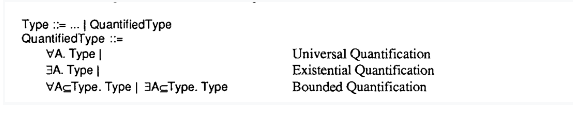
\includegraphics[]{anexos/Screenshot_38.png}
\end{figure}
\par Tipos universalmente quantificados são eles próprios tipos de primeira classe e podem ser parâmetros reais em tal substituição.
A quantificação existencial enriquece os recursos de primeira ordem, permitindo tipos de dados abstratos com representação oculta.